\documentclass[pdf]{beamer}

\usetheme{Warsaw}

\usepackage{alltt}

\usepackage{amssymb, amsmath}

\usepackage[english]{babel}

\usepackage{tikz}
\usetikzlibrary{calc,trees,positioning,arrows,chains,automata,shapes.geometric,%
    decorations.pathreplacing,decorations.pathmorphing,shapes,%
    matrix,shapes.symbols}

\usetikzlibrary{shapes,arrows,automata,positioning,calc}
\usetikzlibrary{fit,backgrounds}
\usetikzlibrary{decorations.pathreplacing}
\tikzset{
>=stealth',
  punktchain/.style={
    rectangle,
    rounded corners,
    % fill=black!10,
    draw=black, very thick,
    text width=6em,
    minimum height=3em,
    text centered,
    on chain},
  line/.style={draw, thick, <-},
  element/.style={
    tape,
    top color=white,
    bottom color=blue!50!black!60!,
    minimum width=8em,
    draw=blue!40!black!90, very thick,
    text width=10em,
    minimum height=3.5em,
    text centered,
    on chain},
  every join/.style={->, thick,shorten >=1pt},
  decoration={brace},
  tuborg/.style={decorate},
  tubnode/.style={midway, right=2pt},
}

% collection of macros used in the paper

%Learners
\newcommand{\learnlib}{LearnLib}

\newcommand{\A}{{\mathcal A}}
\newcommand{\B}{{\mathcal B}}
\newcommand{\CH}{{\mathcal H}}
\newcommand{\M}{{\mathcal M}}
\newcommand{\N}{{\mathcal N}}
\newcommand{\hypoof}[2]{\mathcal{H}(#1,#2)}

\newcommand{\nat}{{\mathbb N}}
\newcommand{\integers}{{\mathbb Z}}

\newcommand{\sem}[1]{[\kern-.5mm[{#1}]\kern-.5mm]}
\newcommand{\eqclass}[1]{[{#1}]}

%DOMAIN AND RANGE
\newcommand{\dom}{{\textsf{dom}}}
\newcommand{\ran}{{\textsf{ran}}}

\newcommand{\natplus}{\nat^{>0}}
\newcommand{\realsplus}{{\mathbb R}^{\geq 0}}
\newcommand{\delays}{{\mathbb R}^{> 0}}
\newcommand{\stoptimer}{\mathit{kill}}
\newcommand{\tosymbol}{\mathit{to}}
\newcommand{\toevent}[1]{\mathit{to}[#1]}
\newcommand{\toevents}{\mbox{\sl TO}}
\newcommand{\extinputs}{\hat{I}}
\newcommand{\Head}[1]{\mathsf{Head}({#1})}
\newcommand{\Tail}[1]{\mathsf{Tail}({#1})}
\newcommand{\Last}[1]{\mathsf{Last}({#1})}
\newcommand{\expirable}{\mathit{expirable}}
\newcommand{\tvals}{\kappa}
\newcommand{\Vals}[1]{\mathit{Val}({#1})}
\newcommand{\delay}[2]{d_{[#1:#2]}}
\newcommand{\timerof}[2]{x_{#1}^{#2}}
\newcommand{\Post}{\mathsf{Post}}
\newcommand{\beh}{\mathit{beh}}
\newcommand{\untime}{\mathit{untime}}
\newcommand{\run}{\mathit{pullback}}
\newcommand{\timedword}{\mathit{tw}}
\newcommand{\timedinputword}{\mathit{tiw}}
\newcommand{\untimedinputword}{\mathit{uiw}}
\newcommand{\startedby}{\mathit{startedby}}
\newcommand{\Mealy}{\mathit{Mealy}}
\newcommand{\finitesubsets}[1]{{\mathcal{P}}_{\mathit{fin}}(#1)}
\newcommand{\conc}{\cdot}
\newcommand{\tuple}[1]{\langle #1\rangle}
\newcommand{\set}[1]{\lbrace #1\rbrace}
\newcommand{\vect}[2]{{#1}_1 , \ldots , {#1}_{#2}}
\newcommand{\setcomp}[2]{\set{#1 ~:~ #2}}
\newcommand{\domof}[1]{\dom(#1)}
\newcommand{\ranof}[1]{\ran(#1)}
\newcommand{\can}[1]{\mathit{can}({#1})}
\newcommand{\uncan}[1]{\mathit{uncan}({#1})}
\newcommand{\zone}[1]{\mathit{Zone}({#1})}
\newcommand{\vars}{\mathcal{X}}
\newcommand{\varsof}[1]{\vars(#1)}
\newcommand{\remap}{\pi}
\newcommand{\remapinst}{\rho}
\newcommand{\constr}{\phi}


\newcommand{\emptyword}{\epsilon}
\newcommand{\lengthof}[1]{|#1|}
\newcommand{\true}{{\it true}}
\newcommand{\false}{{\it false}}

%% macros for ``approximation''
\newcommand{\acttimers}{\mathit{active}}
\newcommand{\constrof}[1]{\phi_{#1}}
\newcommand{\post}{\mathit{post}}

\newcommand{\ctimers}{X}
\newcommand{\normalize}{\gamma}
\newcommand{\normalizeof}[2]{\normalize_{#2}^{#1}}
\newcommand{\timerbij}{\gamma}
\newcommand{\timerequiv}{\pi}
\newcommand{\extendedby}{\lhd}
\newcommand{\uttrace}{\textsf{tr}}
\newcommand{\uttraceof}[1]{\uttrace(#1)}
\newcommand{\uttracesof}[1]{\textsf{Tr}(#1)}
\newcommand{\strace}{\textsf{tr}_s}
\newcommand{\ssuffix}{v_s}
\newcommand{\instancesof}[1]{[\![ #1 ] \! ]}
\newcommand{\suffixbehs}[3]{({#2}^{-1}{#1})\lceil{#3}}
\newcommand{\getmemorable}[3]{\mathit{mem}_{#1,#3}(#2)}
\newcommand{\getassignment}[3]{\mathit{val}_{#1,#3,#2}}
\newcommand{\feasibleinputs}[2]{\mathit{feas}_{#2}(#1)}
\newcommand{\extend}[3]{(#1 \xrightarrow{#2/#3} \emptyset)}
\newcommand{\suffbij}[2]{g_{|#1| \to |#2|}}
\newcommand{\suftraces}{\textsf{Tr}_s}
\newcommand{\pinpof}[1]{\textit{inp}_p(#1)}
\newcommand{\sinpof}[1]{\textit{inp}_s(#1)}
\newcommand{\symbinpof}[1]{\textit{symbinp}(#1)}
\newcommand{\word}{w}
%% \newcommand{\smap}{{\cal O}}
%% \newcommand{\smappre}{{\cal O_p}}
%% \newcommand{\smapsuf}{{\cal O_s}}
%% \newcommand{\obspre}{{\cal O_U}}

\newcommand{\domain}{\mathcal{D}}
\newcommand{\binrelations}{\mathcal{R}}

% Define various macros
\definecolor{darkgreen}{rgb}{0,.75,0}
\definecolor{darkred}{rgb}{.75,0,0}
\definecolor{darkblue}{rgb}{0,0,.75}
\newcommand{\red}[1]{\color{darkred}{#1}\normalcolor }
\newcommand{\green}[1]{\color{darkgreen}{#1}\normalcolor }
\newcommand{\blue}[1]{\color{blue}{#1}\normalcolor }
\newcommand{\tts}{\tt \footnotesize}
\newcommand{\ra}{\rightarrow}

\newif\iflong
%\longtrue
\longfalse

\title[Finding Bugs Using  Automata Learning]{%
Finding Security Vulnerabilities in Protocol Implementations Using Active Automata Learning}

\author[Frits Vaandrager]{%
Frits Vaandrager}

\institute{Radboud University Nijmegen}

\date[]{ICGI, Wroclaw, September 2018}


\beamertemplatenavigationsymbolsempty
%\beamertemplateshadingbackground{red!10}{blue!10}

\begin{document}

\frame{\titlepage}

\section{Introduction}

\frame{
\frametitle{Research Question}

\begin{center}
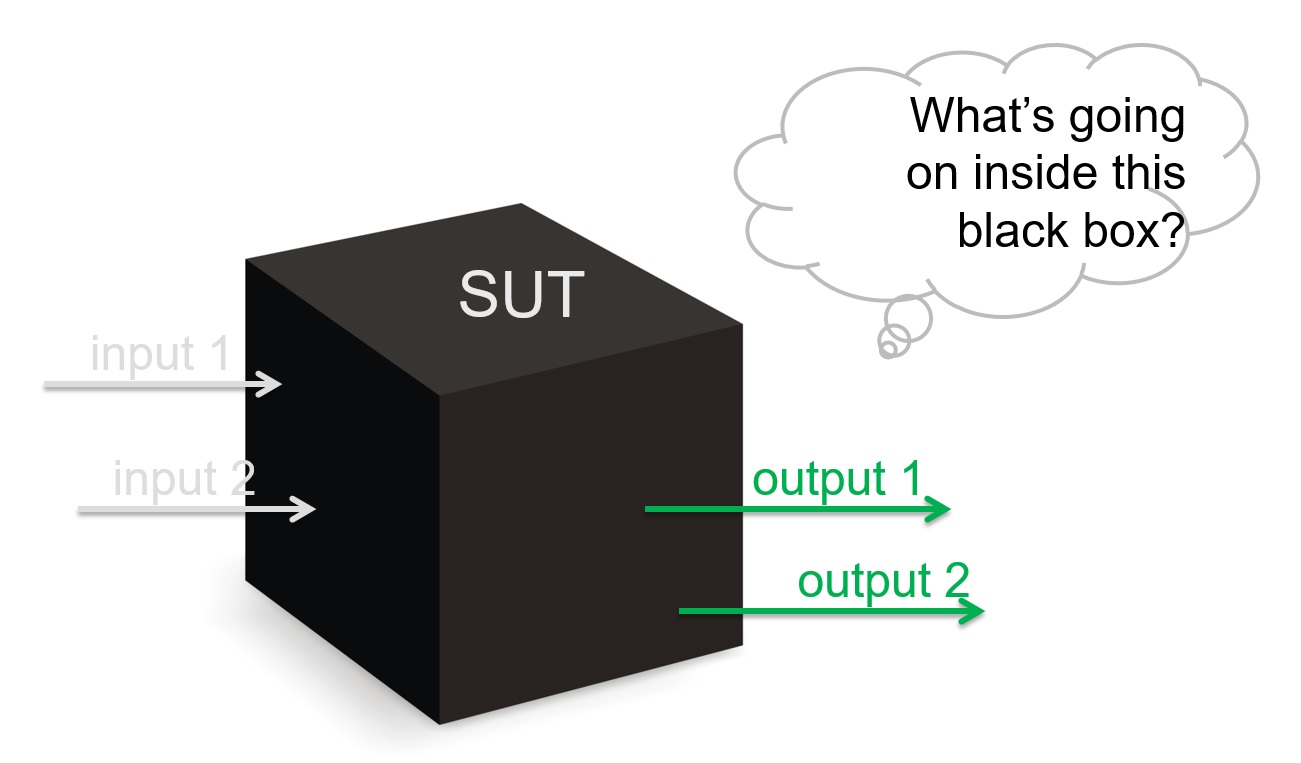
\includegraphics[width=.8\textwidth]{blackbox.jpg}
\end{center}
}

\frame{
\frametitle{Minimally adequate teacher (Angluin)}

\begin{center}
 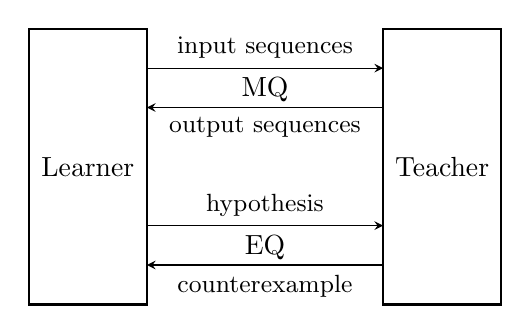
\begin{tikzpicture}[>=stealth]
            \draw [thick] (0,0) rectangle (1.5,3.5) node[midway] {Learner};
            \draw [thick] (4.5,0) rectangle (6,3.5) node[midway] {Teacher};
            \draw [->] (1.5,3) -- (4.5,3) node[midway,below] {MQ};
            \draw (1.5,3) -- (4.5,3) node[midway,above] {\small input sequences};
            \draw [<-] (1.5,2.5) -- (4.5,2.5) node[midway,below] {\small output sequences};
            \draw [->] (1.5,1) -- (4.5,1) node[midway,below] {EQ};
            \draw (1.5,1) -- (4.5,1) node[midway,above] {\small hypothesis};
            \draw [<-] (1.5,0.5) -- (4.5,0.5) node[midway,below] {\small counterexample};
        \end{tikzpicture}
        \hspace{2 em}
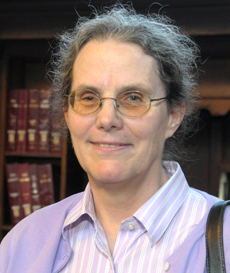
\includegraphics[width=.25\textwidth]{angluin.png}
\end{center}
}
\frame{
\frametitle{Black box checking (Peled, Vardi \& Yannakakis)}

\begin{center}
 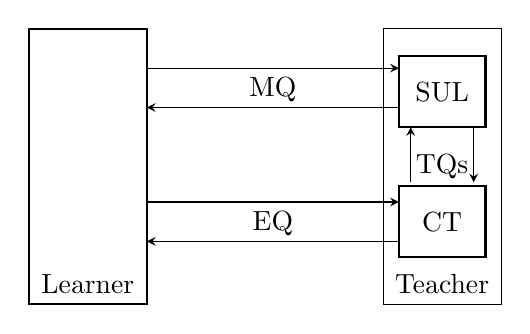
\begin{tikzpicture}[>=stealth]
            \draw [thick] (0,0) rectangle (1.5,3.5);
            \draw (4.5,0) rectangle (6,3.5) node[midway] {TQs};
            \draw [thick] (4.7,2.25) rectangle (5.8,3.15) node[midway] {SUL};
            \draw [thick] (4.7,0.6) rectangle (5.8,1.5) node[midway] {CT};
            \draw [->] (1.5,3) -- (4.7,3) node[midway,below] {MQ};
            \draw [<-] (1.5,2.5) -- (4.7,2.5);
            \draw [->] (1.5,1.3) -- (4.7,1.3) node[midway,below] {EQ};
            \draw [<-] (1.5,0.8) -- (4.7,0.8);
            \draw [->] (4.85,1.55) -- (4.85,2.25);
            \draw [<-] (5.65,1.55) -- (5.65,2.25);
            \node [below] at (0.75,0.5) {Learner};
            \node [below] at (5.25,0.5) {Teacher};
        \end{tikzpicture}
                \hspace{1 em}
        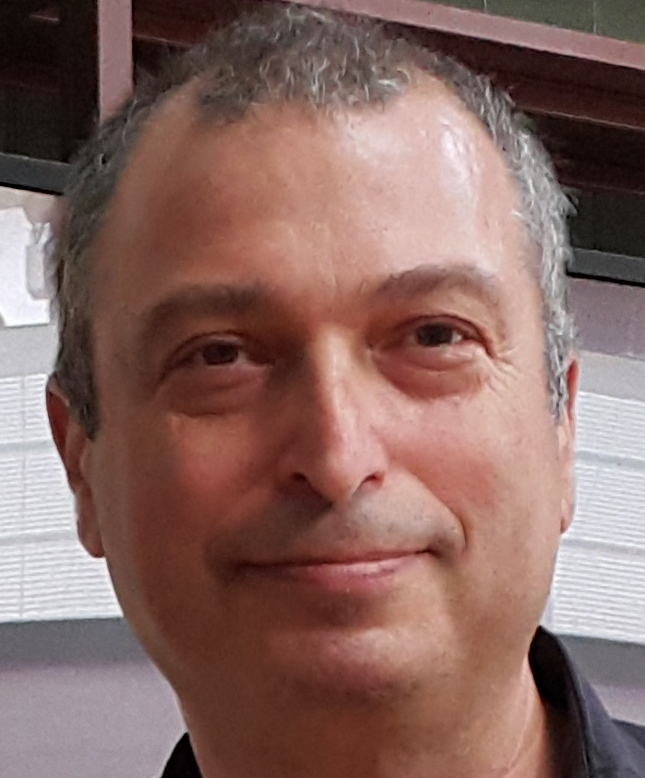
\includegraphics[width=1.2cm]{peled.jpg}
        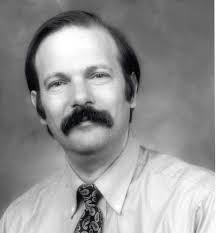
\includegraphics[width=1.35cm]{vardi.jpeg}
        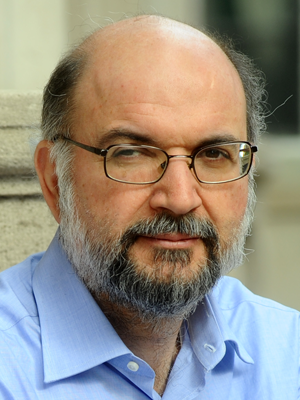
\includegraphics[width=1.1cm]{Yannakakis.png}
\end{center}
\red{Learner}: Formulate hypotheses\\
\red{Conformance Tester (CT)}: Test correctness hypotheses


\pause
\vspace{0.5em}
\red{Model learning and conformance testing two sides of same coin!}
}

\frame{
\frametitle{LearnLib}

\begin{center}
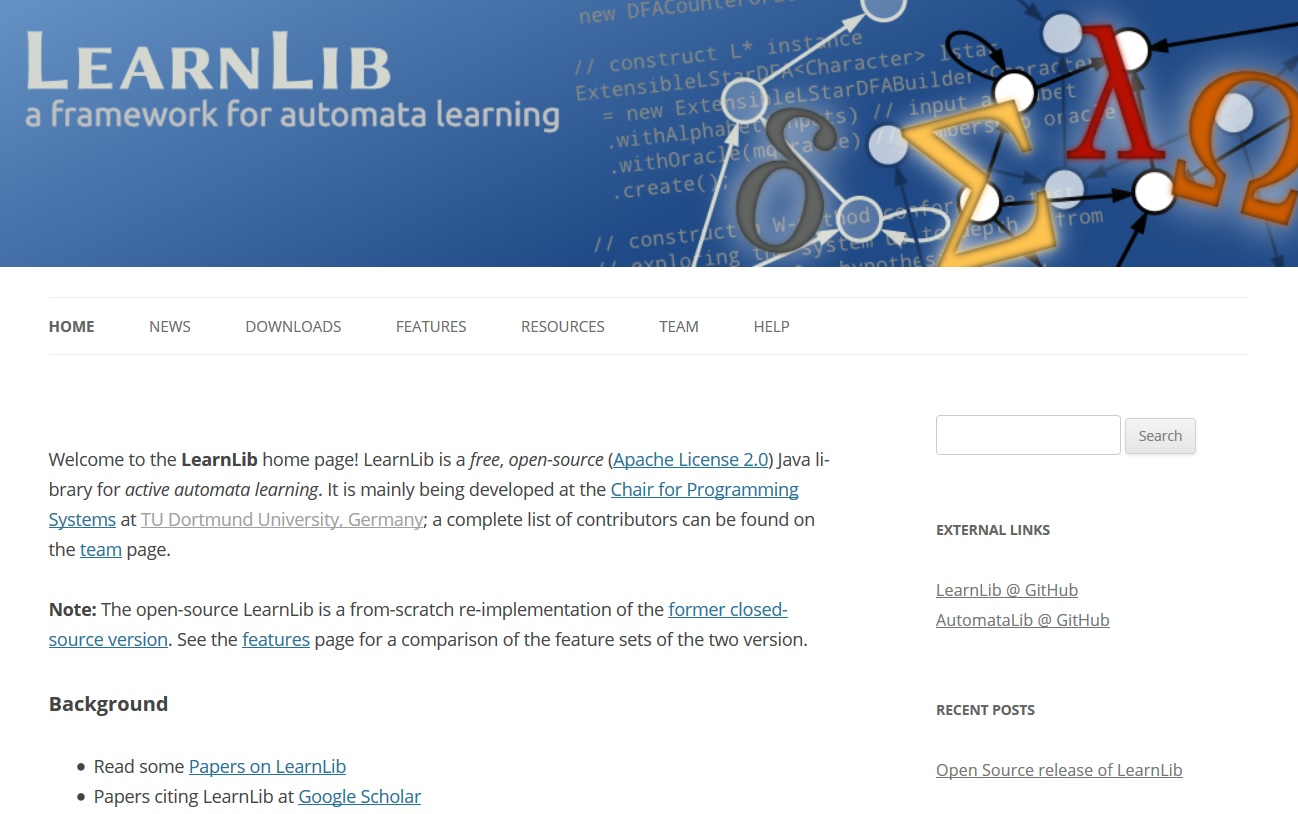
\includegraphics[width=.7\textwidth]{LearnLib.jpg}
    \hspace{1 em}
        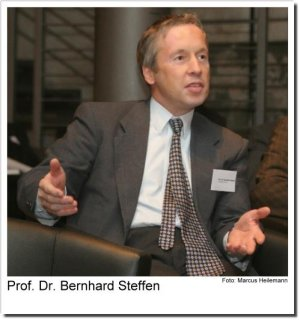
\includegraphics[width=2.5cm]{steffen.jpg}
\end{center}
}

\frame{
\frametitle{Research method (FMSD, 2015)}

\begin{center}
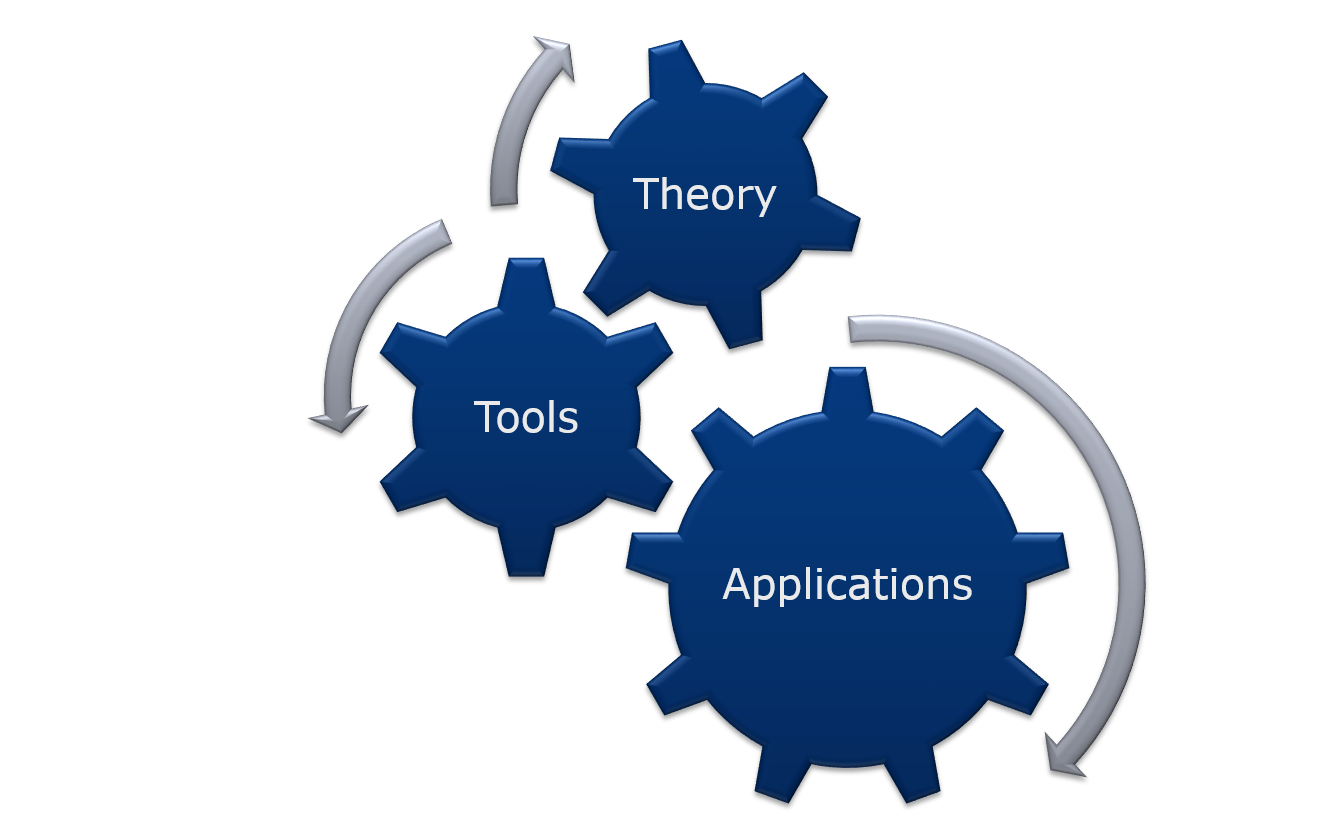
\includegraphics[width=.8\textwidth]{method.png}
\end{center}
}

\frame{
\frametitle{A theory of mappers}

\begin{center}
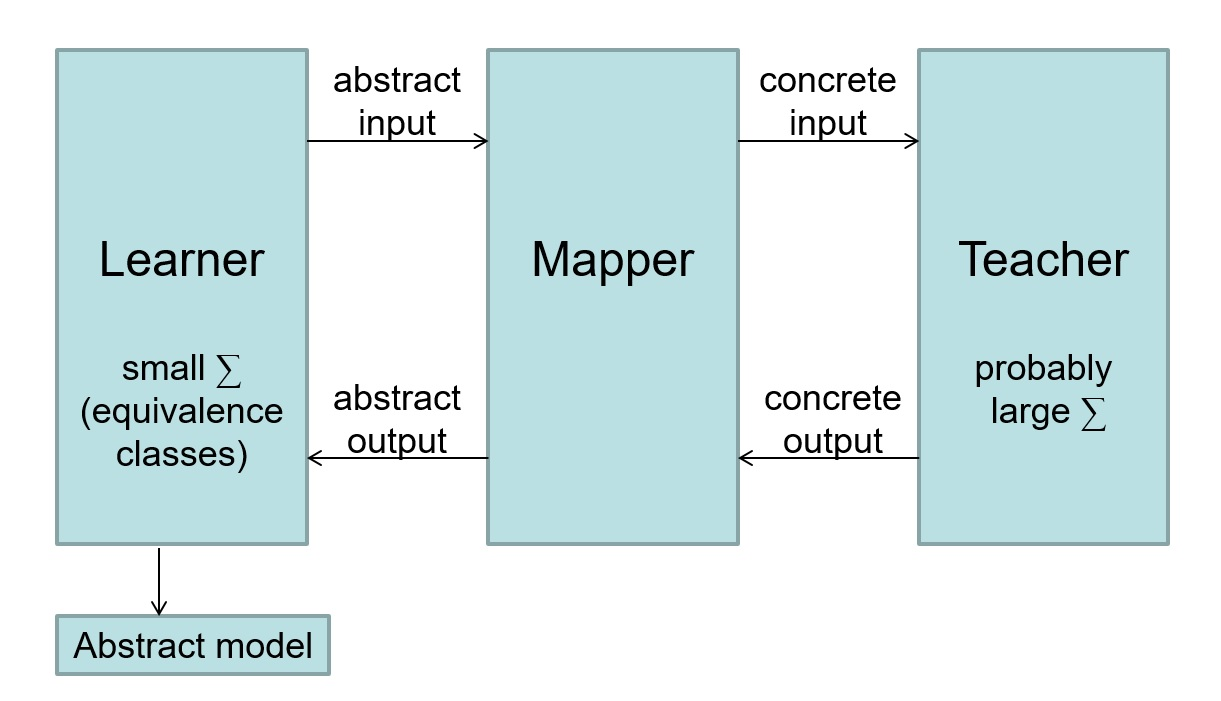
\includegraphics[width=.8\textwidth]{mappers.jpg}
\end{center}
}

\frame{
\frametitle{A theory of mappers (cnt)}

Formally, a mapper can be viewed as a transducer (deterministic Mealy machine). A mapper ${\cal A}$ induces an \red{abstraction operation\ } $\alpha_{\cal A}$ and a \red{concretization\ } operator $\gamma_{\cal A}$.



\begin{theorem}
For a mapper ${\cal A}$ and nondeterministic Mealy machines ${\cal M}$ and ${\cal H}$, $\alpha_{\cal A}({\cal M}) \leq {\cal H}$ implies ${\cal M} \leq \gamma_{\cal A}({\cal H})$
\end{theorem}


\begin{theorem}
Suppose $\alpha_{\cal A}({\cal M})$ has no transitions with output $\perp$.
Then
${\cal M} \leq \gamma_{\cal A}({\cal H})$ implies
$\alpha_{\cal A}({\cal M}) \leq {\cal H}$. 
\end{theorem}
}

\section{Case Studies}

\frame{
\frametitle{EMV protocol (Aarts et al, 2013)}

\begin{columns}
\begin{column}{0.5\textwidth}
    \begin{center}
     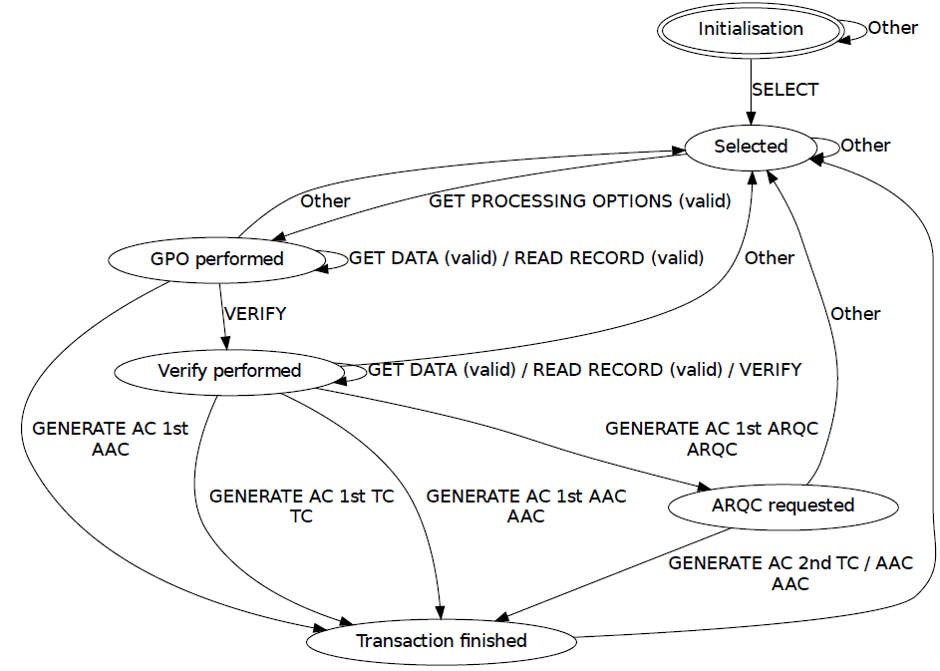
\includegraphics[width=\textwidth]{EMV.png}
     \end{center}
\end{column}
\begin{column}{0.5\textwidth}
{\small
\begin{itemize}
\item 
EMV = Europay/Mastercard/Visa
\item
Compatibility between smartcards and terminals 
\item
SEPA requires EMV compliance
\item
EMV standard has $>$700 pages
\item
Learning took at most 1500 membership queries, less than 30 minutes
\item
Useful for fingerprinting cards
\end{itemize}
}
\end{column}
\end{columns}
}
\frame{
\frametitle{E.dentifier2 (WOOT'14)}
\begin{center}
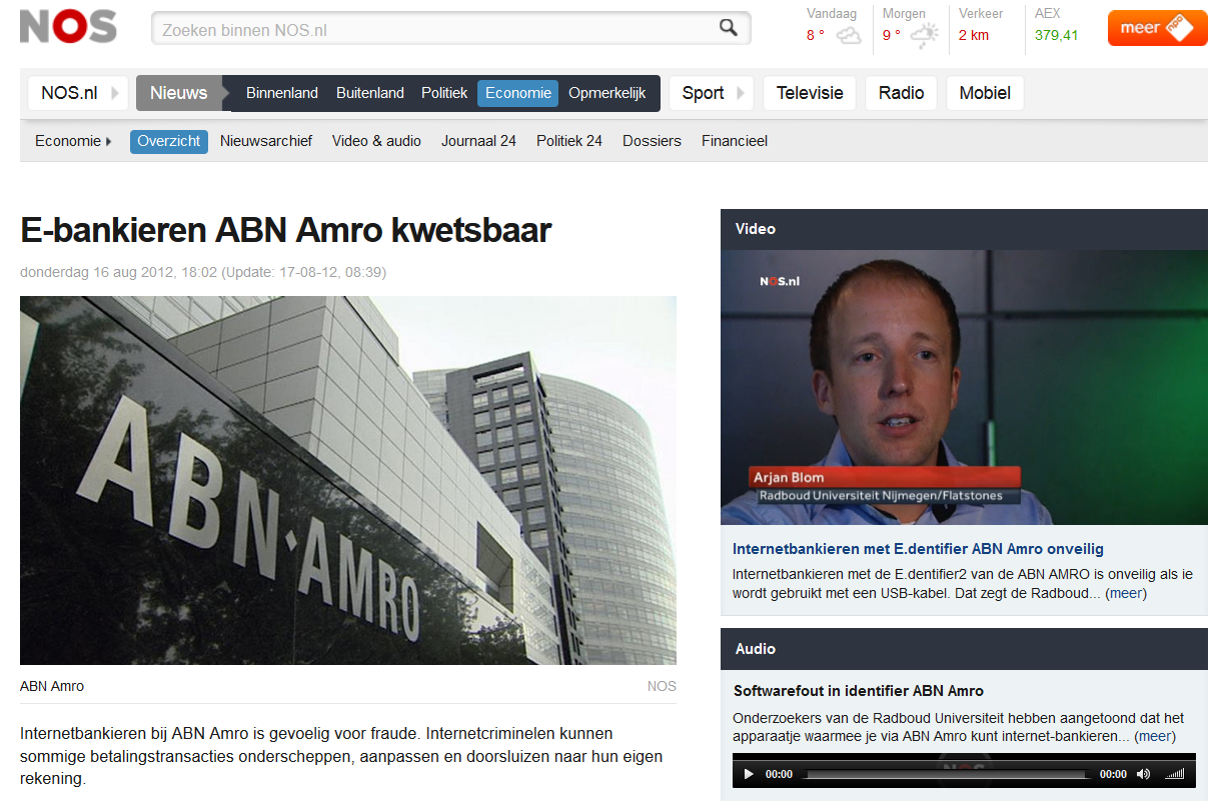
\includegraphics[width=.8\textwidth]{nosedentifier.png}
\end{center}
}

\frame{
\frametitle{State machines for old and new E.dentifier2}
\begin{center}
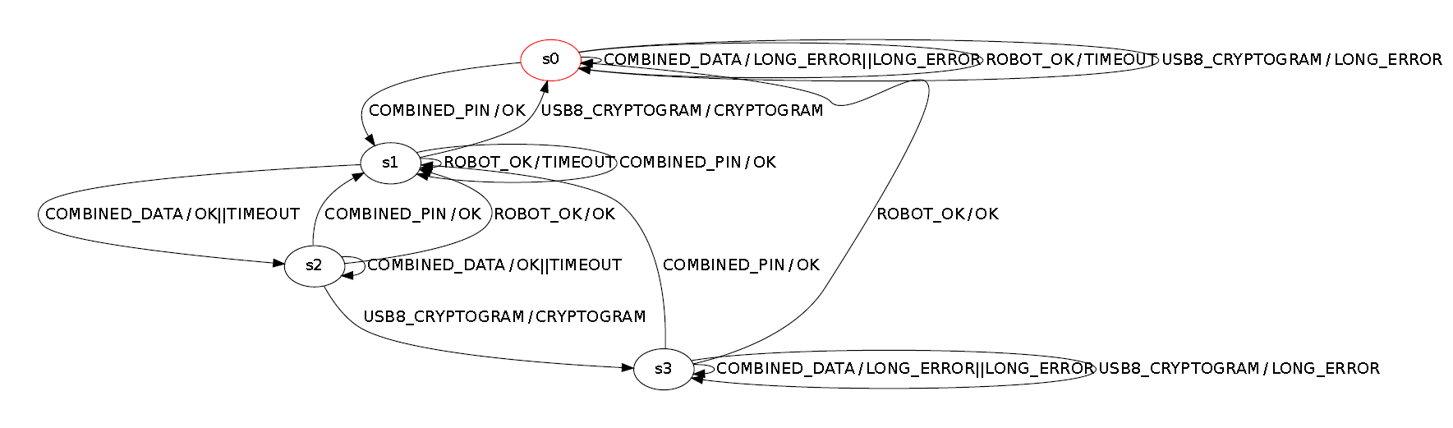
\includegraphics[width=.9\textwidth]{oldedentifier.png}

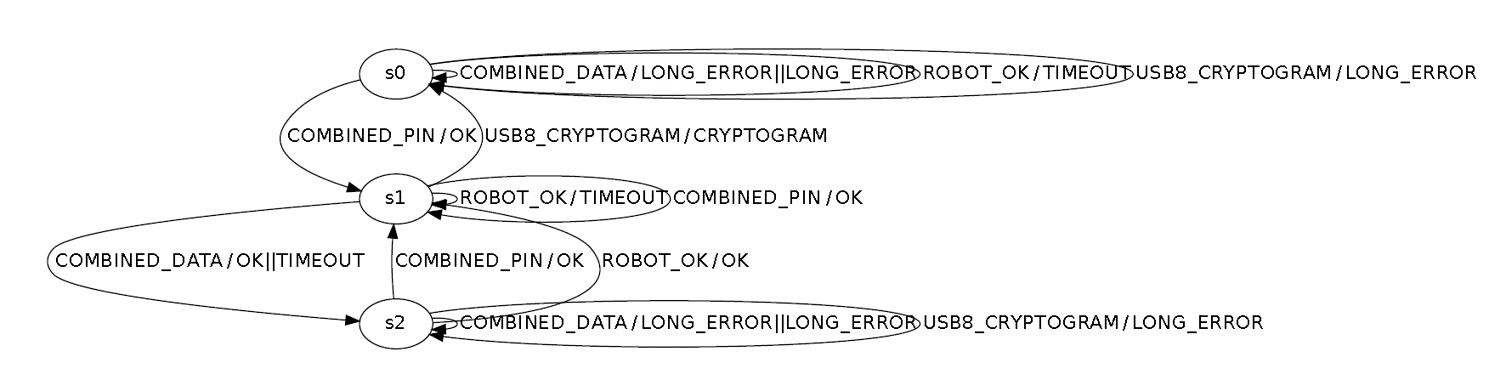
\includegraphics[width=.9\textwidth]{newedentifier.png}
\end{center}
}

\frame{
\frametitle{Bugs in protocol implementations}

\begin{columns}
\begin{column}{0.5\textwidth}  %%<--- here
    \begin{center}
     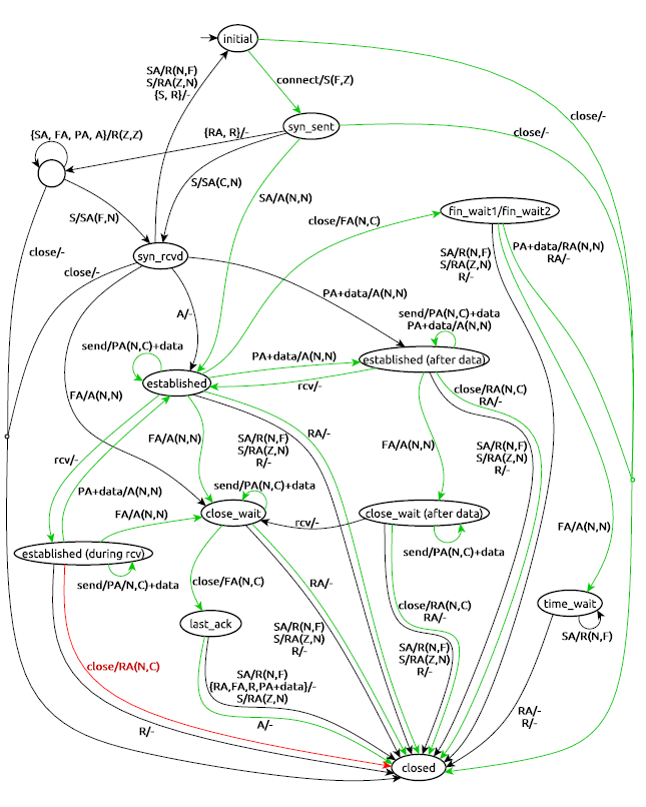
\includegraphics[width=0.9\textwidth]{TCPbug.png}
     \end{center}
\end{column}
\begin{column}{0.5\textwidth}
Standard violations found in implementations of major protocols: 
\begin{itemize}
\item
\blue{TLS}\  (Usenix Security'15)
\item 
\blue{TCP}\  (CAV'16)
\item
\blue{SSH}\  (Spin'17).
\end{itemize}
%
\pause
\red{These findings led to bug fixes in implementations.}
\end{column}
\end{columns}

}

\frame{
\frametitle{Learned model for SSH implementation}

\begin{center}
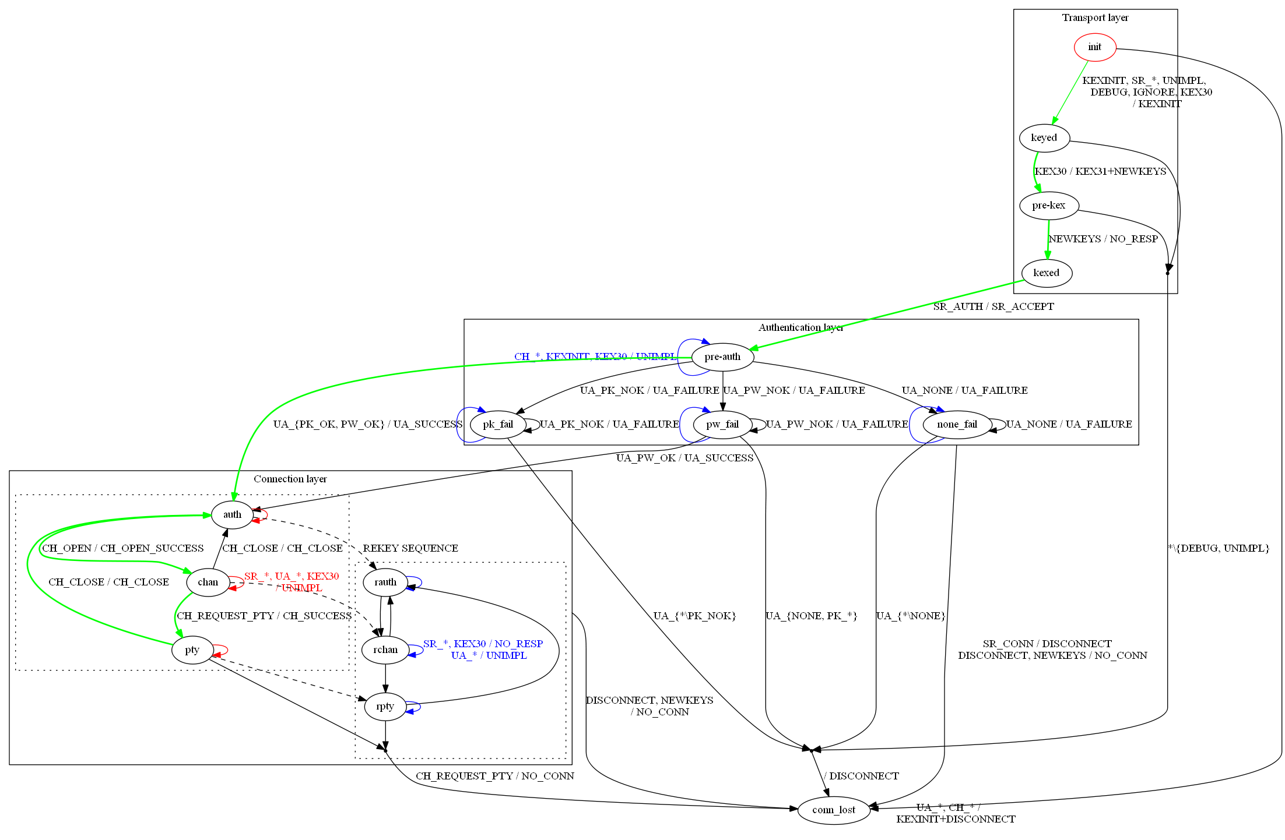
\includegraphics[width=.8\textwidth]{sshbug.png}
\end{center}
}
\frame{
\frametitle{SSH model checking results}

\begin{center}
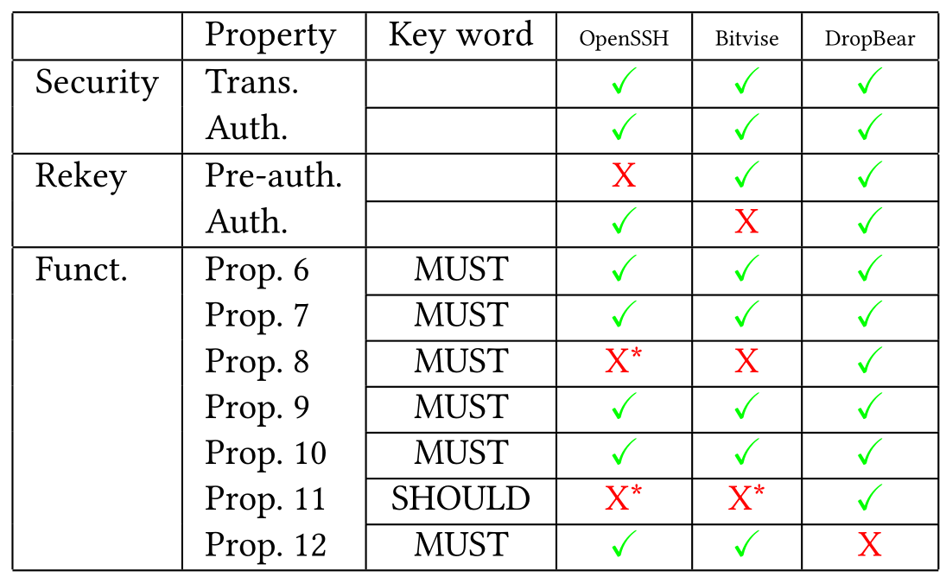
\includegraphics[width=.8\textwidth]{sshresults.png}
\end{center}
}

\frame{
\frametitle{Other case studies}
\begin{itemize}
\item
Session Initiation Protocol (SIP)
\item
Message Queuing Telemetry Transport (MQTT) protocol
\item
Quick UDP Internet Connections (QUIC) protocol
\item
WiFi
\item
IEC 60870-5-104 protocol
\item
...
\end{itemize}
}

\frame{
\frametitle{Lorentz Workshop}

\begin{columns}
\begin{column}{0.5\textwidth}  %%<--- here
    \begin{center}
     \includegraphics[width=\textwidth]{lorentz.jpg}
     \end{center}
\end{column}
\begin{column}{0.5\textwidth}
Participants from automata learning, model-based testing, cryptography, and security protocol implementation. 

\vspace{0.5em}
Working groups on e.g.,
   \begin{itemize}
   \item 
   WiFi
   \item
   side channels in TLS
   \item
   LTE
   \end{itemize}
\end{column}
\end{columns}
}

\frame{
\frametitle{Automata wiki}

\begin{center}
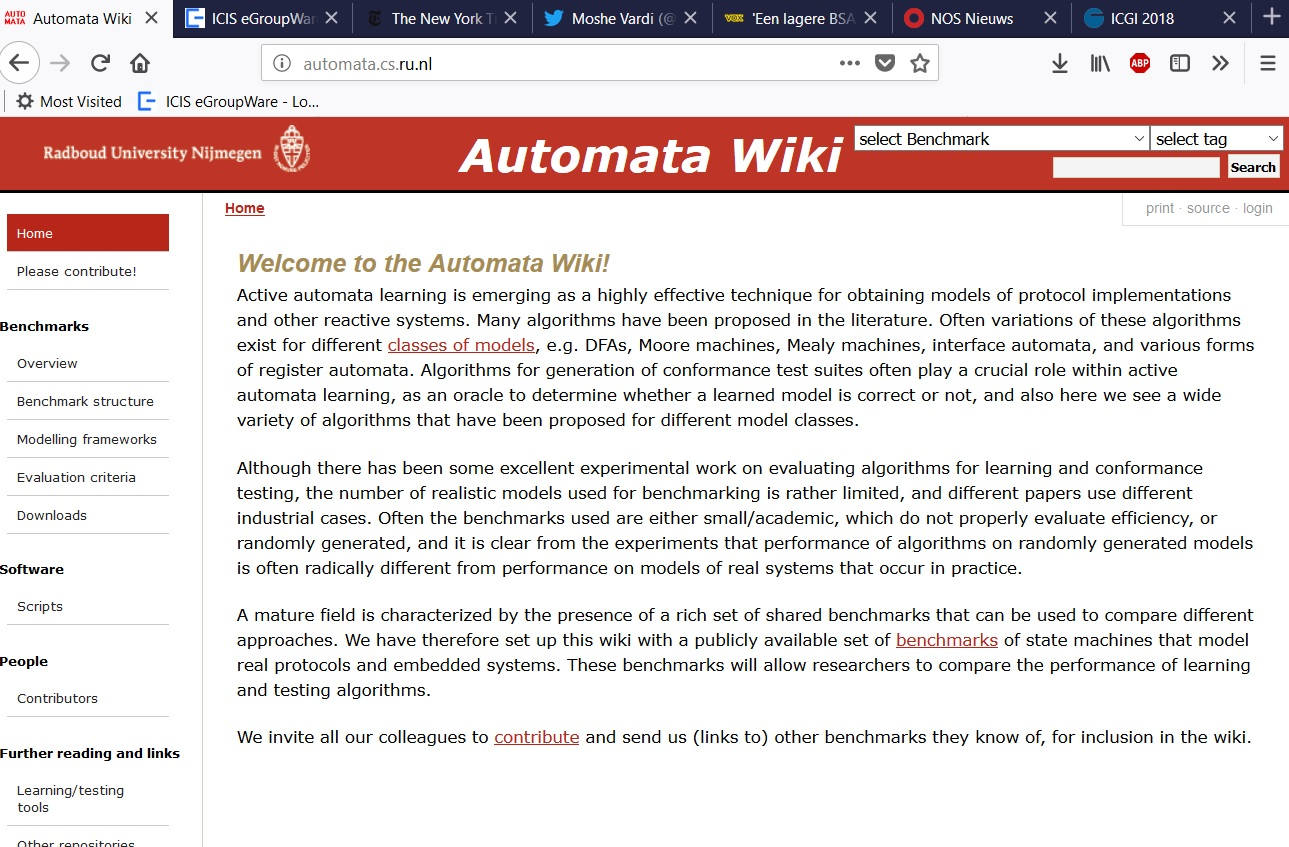
\includegraphics[width=.9\textwidth]{automatawiki.jpg}
\end{center}
}


\frame{
\frametitle{Automata wiki}

\begin{center}
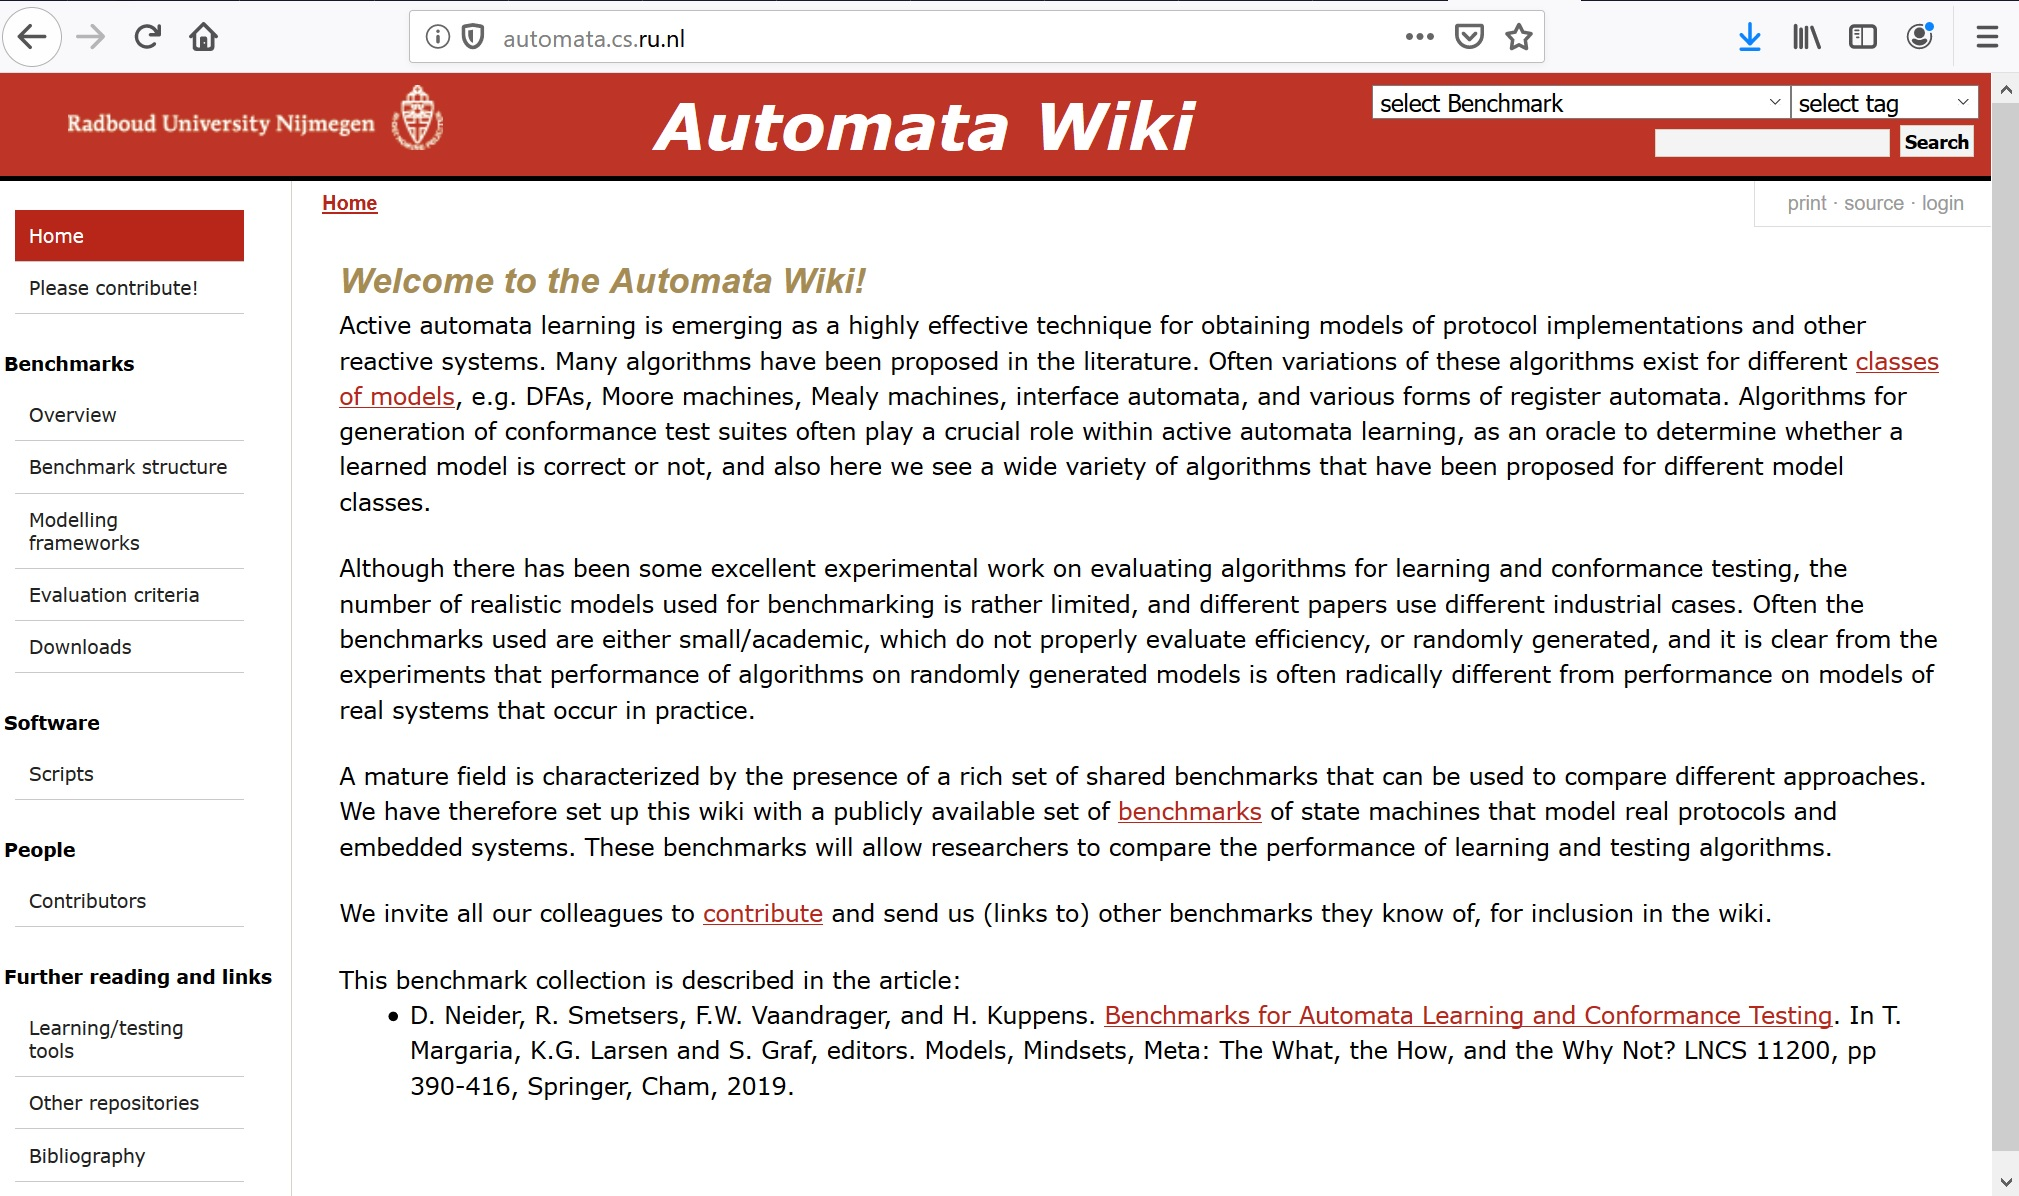
\includegraphics[width=.9\textwidth]{benchmarks.jpg}
\end{center}
}


\frame{
\frametitle{Automata wiki: supported automata frameworks}

\begin{center}
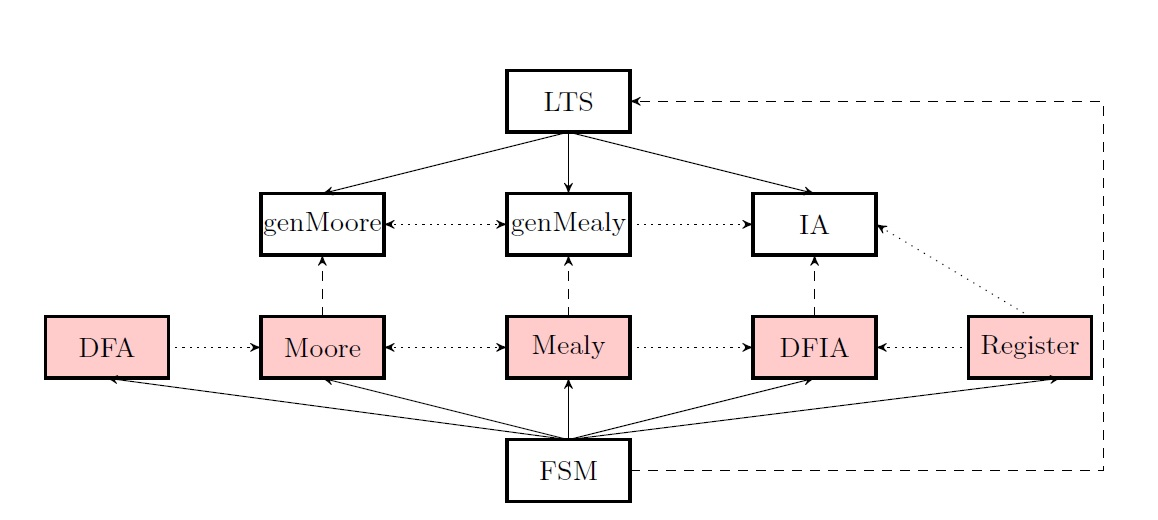
\includegraphics[width=.9\textwidth]{automataframeworks.jpg}
\end{center}
}


\frame{
\frametitle{Automata wiki: most benchmarks are not that big}

\begin{center}
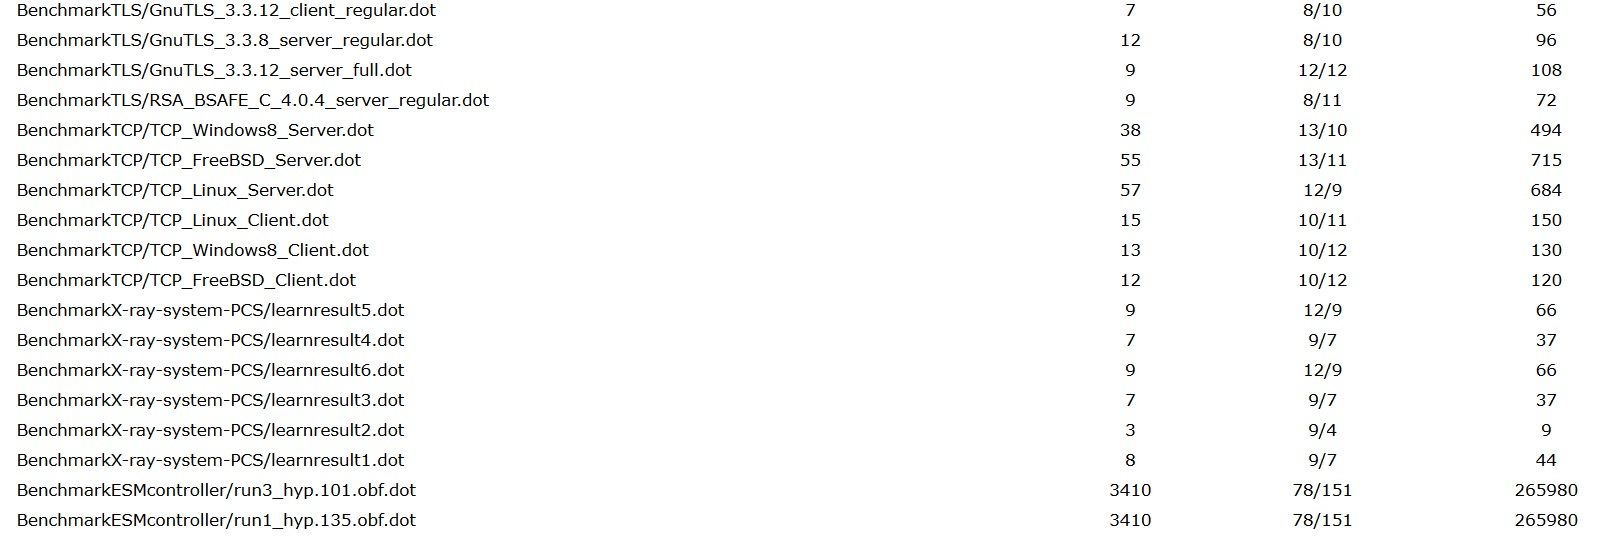
\includegraphics[width=\textwidth]{benchmarksize.jpg}
\end{center}
}

\section{Register Automata}
\frame{
\frametitle{Register automata}

Actions may carry data parameters that may be stored in registers:
\begin{center}
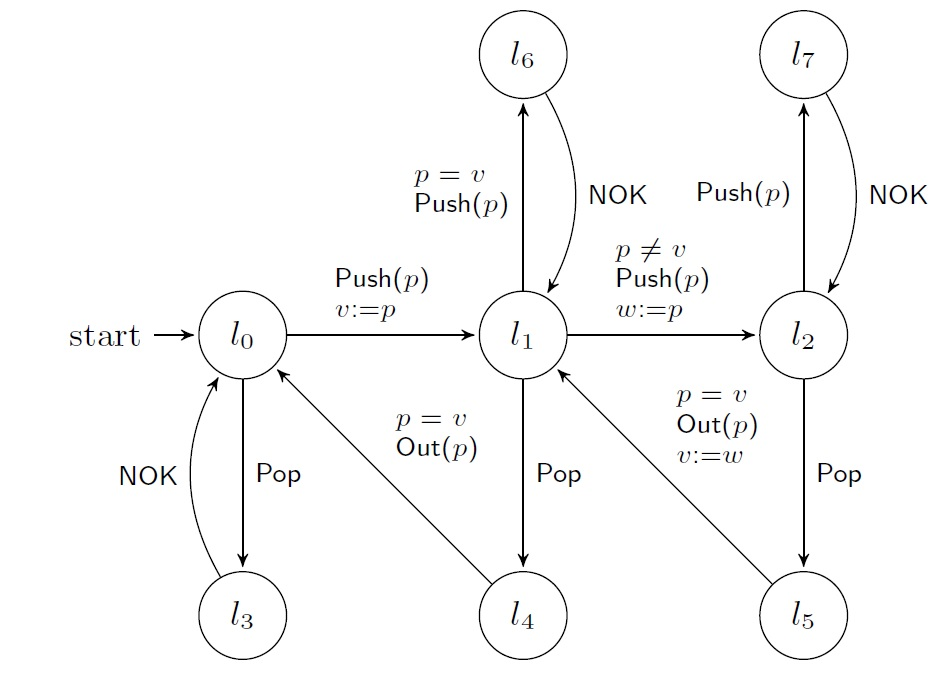
\includegraphics[width=.8\textwidth]{fifoset.jpg}
\end{center}
}

\frame{
\frametitle{Data types}

Register automata may be parametrized by a \red{(relational) structure}: a pair $\tuple{\domain, \binrelations}$
where $\domain$ is an unbounded domain
% \todobj{Do we need it to be unbounded?}
of \red{data values}, and
$\binrelations$ is a collection of \red{relations\ } on $\domain$. 

\vspace{0.5em}
Examples of simple structures include:
\begin{itemize}
\item
  $\tuple{\mathbb{N}, \{=\} }$, the natural numbers with
  equality; 
\item
  $\tuple{\mathbb{R}, \{ <\} }$, the real numbers with inequality:
  this structure also allows one to express equality between elements.
\end{itemize}
Transition guards are conjunctions of negated and unnegated relations from $\binrelations$.
}

\frame{
\frametitle{Learning tools for register automata}
\begin{itemize}
\item 
\blue{Tomte}, Radboud University, can only handle $\tuple{\mathbb{N}, \{=\} }$
\item
\blue{LearnLib}, TU Dortmund, can only handle $\tuple{\mathbb{N}, \{=\} }$
\item
\blue{RALib}, Uppsala/Dortmund, can handle some richer structures
\end{itemize}

}
\frame{
\frametitle{TCP protocol case study (FMICS-AVoCS'17)}

\begin{center}
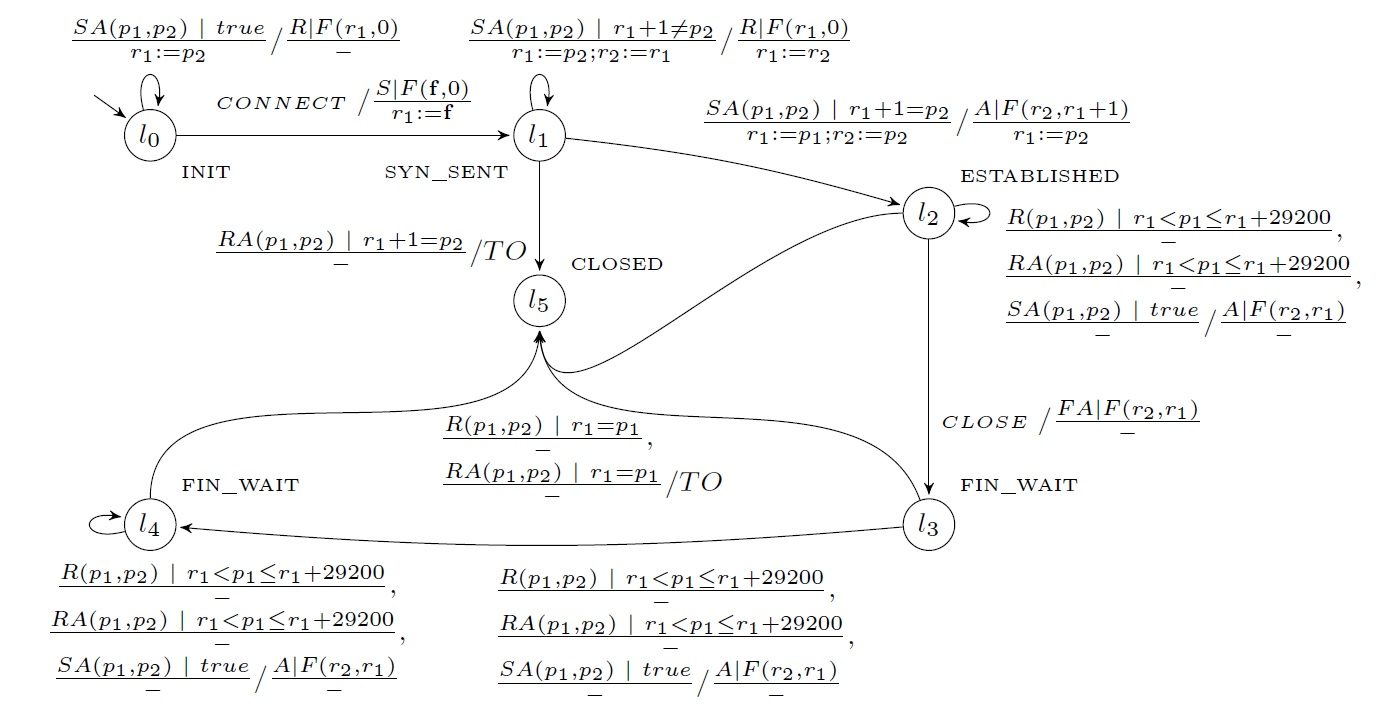
\includegraphics[width=\textwidth]{TCPlinux.jpg}
\end{center}
\pause
\red{These findings led to bug fix in Linux TCP implementation.}
}

\section{Taint Analysis}

\frame{
\frametitle{Limits of black-box learning?}

\begin{itemize}
\item 
Model learning is an highly effective bug finding technique
\pause
\item
... but it has some serious scalability problems
\pause
\item
\red{Can we use white-box information while preserving the extensionality of black-box models?}
\end{itemize}
}

\frame{
\frametitle{Idea: Use Taint Analysis}

\begin{center}
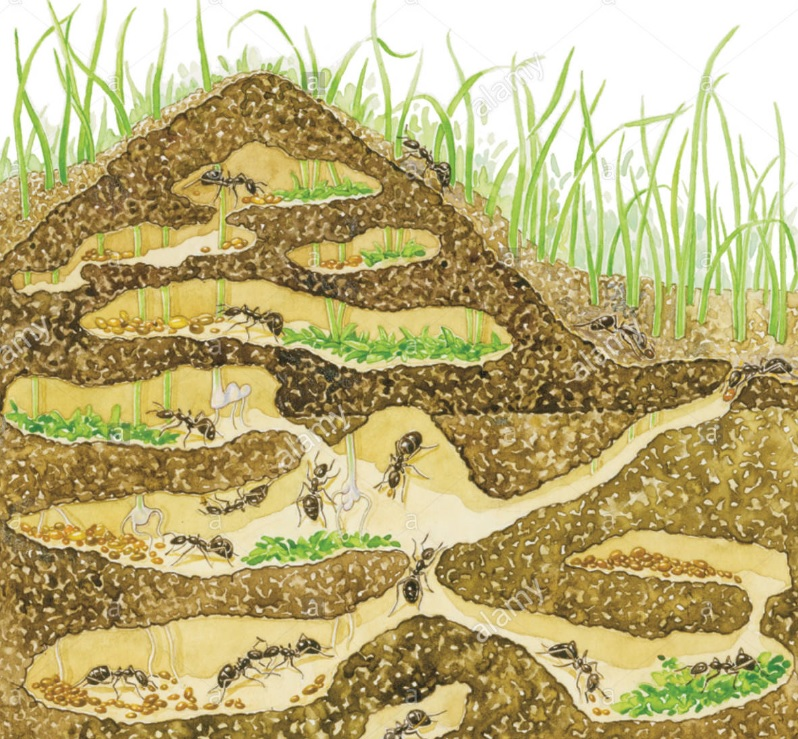
\includegraphics[width=.8\textwidth]{ants.jpg}
\end{center}
}


\frame{
\frametitle{Taint Analysis}

\begin{itemize}
\item
White-box technique for code analysis
\item
Instruments code to track input values
\item
Many tools focus on specific vulnerabilities, e.g.\ buffer overflows and sql injections
\item
Usually implemented using Dynamic Binary Analysis, e.g.\ Valgrind
\item
We use Python library from Pygmalion tool from Andreas Zeller et al.
\end{itemize}
}

\frame{
\frametitle{What Does Pygmalion Tool Do For Us?}

\begin{center}
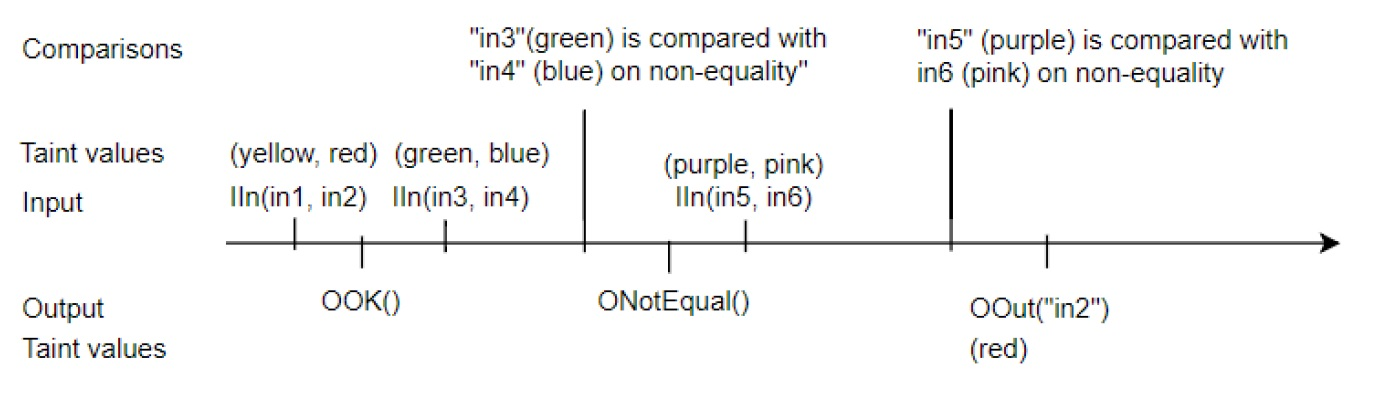
\includegraphics[width=\textwidth]{taintedtrace.jpg}
\end{center}

\pause
\red{Potential of exponential gains during learning!}
}
\frame{
\frametitle{Architecture RAlib Tool for Learning Register Automata}

\begin{center}
 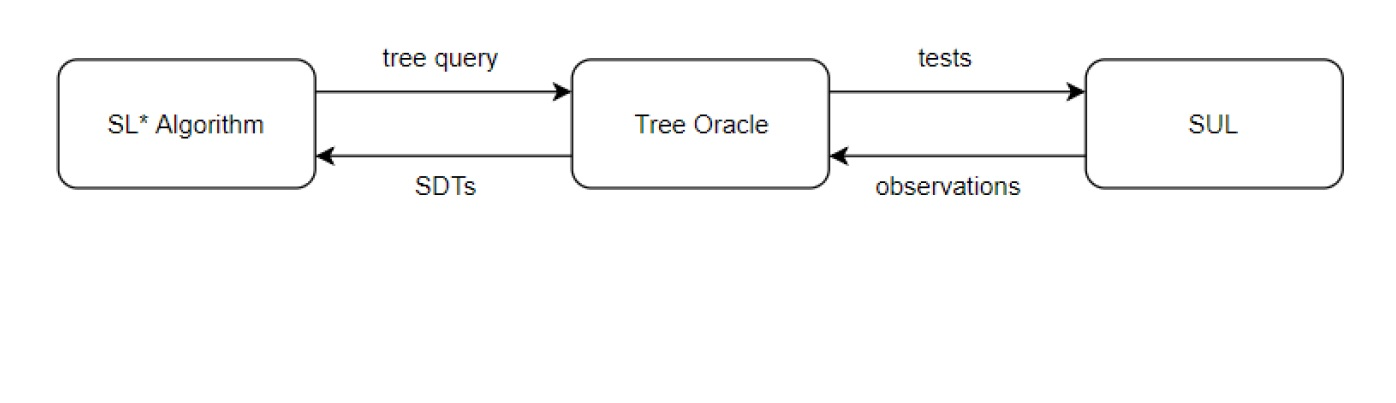
\includegraphics[width=\textwidth]{ralib.jpg}
\end{center}
}

\frame{
\frametitle{Tree Oracle}

\begin{center}
 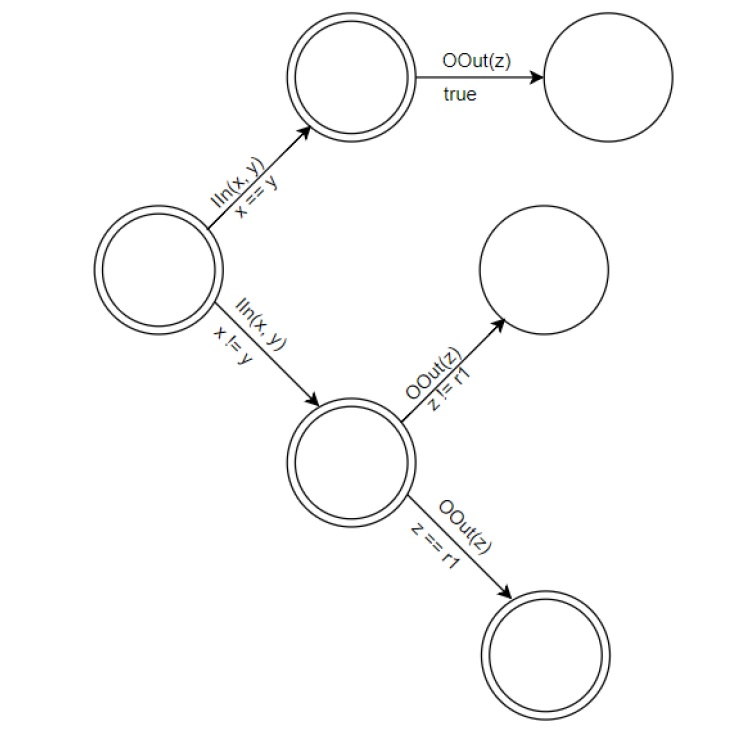
\includegraphics[width=0.6\textwidth]{SDT.jpg}
\end{center}
}

\frame{
\frametitle{Ongoing Work}

Replace tree oracle in RAlib by a version that uses taint analysis.

\vspace{2cm}
\pause
\red{First prototype finished (for integers with equality)!!!}
}

\section{Conclusions and Future Work}
\frame{
\frametitle{Conclusion}
Active automata learning is emerging as a highly effective bug-finding technique,
and slowly becoming a standard tool in the toolbox of the software engineer.

\vspace{1 em}
But \red{much\ } further research is needed!
}

\frame{
\frametitle{Future Work}
\begin{enumerate}
\item
Explore combinations of black-box and white-box learning
\item
Further improvement of learning and testing algorithms for FSM models
\item
Develop algorithms for models with time and probabilities
\item
Refactoring of legacy software is potentially excellent application domain
\item
Please contribute benchmarks to our repository!
\end{enumerate}
}





\end{document}
